\documentclass[a4paper,11pt]{article}
\usepackage[spanish, activeacute]{babel}

\addtolength{\topmargin}{-80pt}
\addtolength{\textwidth}{170pt}
\addtolength{\textheight}{145pt}
\addtolength{\oddsidemargin}{-80pt}

\usepackage{graphicx} % para incluir graficos
\usepackage{amsmath} 
\usepackage{amsthm} % para escribir teoremas lindos
\usepackage{amsfonts} % para tener el simbolo de los numeros reales
\usepackage{color}  % colores de las fuentes

\theoremstyle{definition} \newtheorem{axiom}{Axioma}

\begin{document}
\newcommand{\Nat}{\mathbb{N}}
\newcommand{\cita}{\textcolor{red}{cita}}
\newcommand{\alert}[1]{\textcolor{red}{#1}}
\newcommand{\comment}[1]{\textcolor{blue}{#1}\newline}
%\renewcommand{\comment}[1]{\ }
\theoremstyle{definition} \newtheorem{definition}{Definici'on}

\tableofcontents

\input{abstract}
\section{Introducci\'on y objetivos}
Hacia fines del siglo XIX y principios del siglo XX (\alert{revisar}), con el prop'osito de estudiar la estructura interna de una pieza musical, 
Heinrich Schenker elabor'o una teor'ia de la coerencia tonal en la m'usica conocido como \texttt{an'alisis schenkeriano}.
En su teor'ia, Schenker postula que la superficie musical (lo que se escucha) es resultado de sucesivas transformaciones que sufre una estructura b'asica fundamental 
denominada por el autor la \emph{ursatz}\footnote{estructura fundamental en alem'an}. Estas transformaci'ones estan descriptas en t'erminos de reglas de reescritura que permiten 
a partir de una cierta ursatz llegar a una pieza musical competa. Dado que la ursatz es la estructura fundamental, 'esta s'olo contiene las notas que dan la impronta de la pieza, 
que luego son elaboradas usando las reglas de reescritura.

Si bien el an'alisis schenkeriano fue concebido para llevar la ursatz a una pieza musical completa, queda claro que se lo puede utilizar tambi'en para estimar
cual podr'ia ser la ursatz de un cierta superficie musical. De esta forma, al utilizar la teor'ia ``en sentido contrario'', en vez de hablar en t'erminos de elaboraci'ones de 
la ursatz a la superficie musical, habr'ia que hacerlo en terminos de reducciones. Definida como lo opuesto a una elaboraci'on, una reducci'on permite especificar que una cierta 
nota dentro de un grupo es la estructuralmente mas importante, y que todo el resto es una \texttt{elaboraci'on} de esta. 
Dado que esta relaci'on de reducci'on/elaboraci'on se puede aplicar recursivamente, naturalmente emerge una relaci'on 
jer'arquica entre las notas de una pieza musical.  En esta jerarqu'ia, el nivel m'as bajo es lo que se encuentra escrito en la partitura, y a medida que se sube de nivel se 
encuentra la misma pieza musical, pero carente de elaboraciones. En la figura \ref{fig_analisis_schenkeriano} se exhibe un ejemplo de dicho an'alisis.


\begin{figure}[h]
\begin{center}
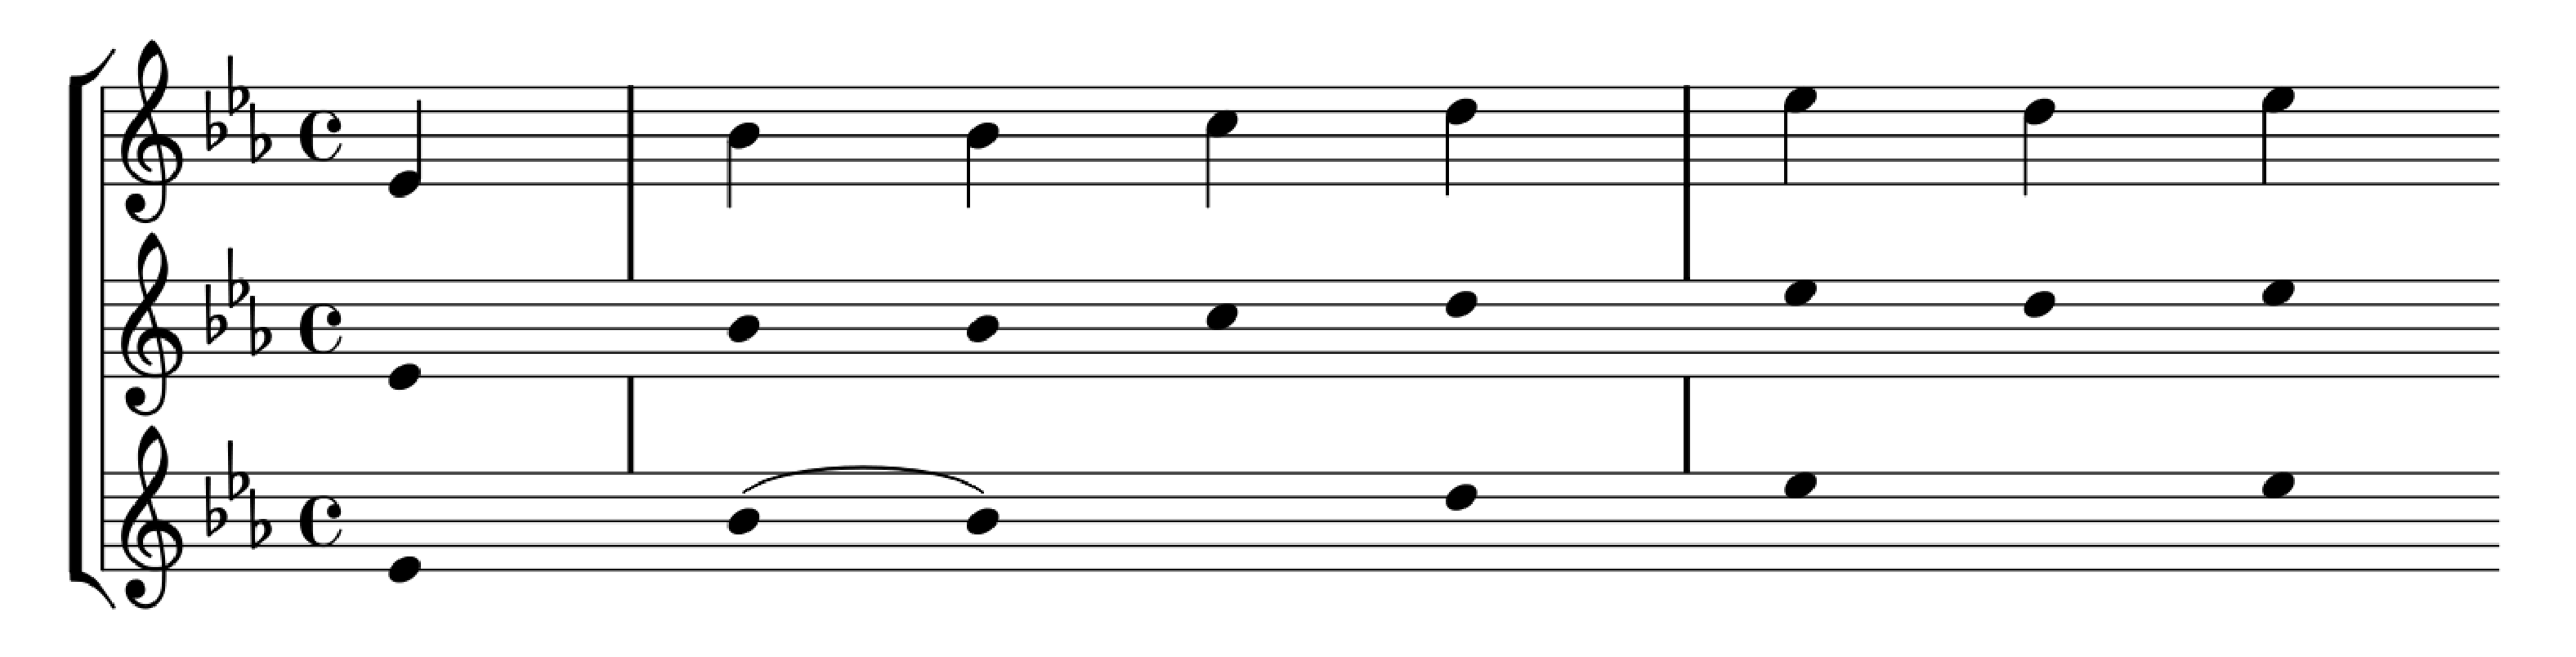
\includegraphics[width=12cm]{images/schenkerian_example}
\label{fig_analisis_schenkeriano}
\newline \alert{poner una imagen mas copada}
\end{center}
\end{figure}

En esta figura, los sucesivos pentagramas muestran relaciones de reducci'on, as'i simplificando el tema con el objeto de llevarlo a una representaci'on m'as abstracta.

El parecido de este tipo de relaciones con las relaci'ones utilizadas por Noam Chomsky para analizar el lenguaje natural es notable. 
Si bien en la teor'ia de Chomsky las relaciones son relaciones del tipo ``es un'', y en la teor'ia de Schenker son del tipo ``es una elaboraci'on de'', 
estas se enmarcan matem'aticamente en el mismo lugar.  

En 1983, el m'usico Fred Lerdahl y el ling\"uista Ray Jackendoff publicaron el libro 
\texttt{A Generative Theory of Tonal Music}(GTTM) donde proponen una gram'atica para analizar la m'usica t'erminos parecidos a los de Schenker. 
Lo interesante de este trabajo es el fundamento que se le da a la elecci'on de las reglas de la gram'atica, puesto que proponen una teor'ia que tomando los conceptos claves
de la teor'ia schenkeriana se basa en supuestos cognitivos de naturaleza computacional.

El objetivo del trabajo de Lerdahl y Jackendoff es principalmente tener modelizar el proceso mediante el cual se estructura la percepci'on de la m'usica. 
Este modelo consiste en una serie de reglas de preferencia. Cada regla tiene asociado un predicado booleano $P$ y un valor de preferencia $v$, 
de modo que si el predicado booleano es verdadero, entonces aportan $v$ unidades a la preferencia de una cierta acci'on interpretativa. Para ejemplificar, a continuaci'on se cita
una regla de preferencia de los autores. Esta regla es una de las reglas asociadas a lo que los autores llaman agrupamiento, que b'asicamente consiste en agrupar notas que tienen
significancia de frase\footnote{M'as adelante se explicar'a esto con mayor detalle}.
\newline

\begin{center}
\texttt{GPR 1} Evite fuertemente grupos que contengan solamente un evento.
\end{center}

En este caso, el predicado booleano es aquel que es verdadero solamente con grupos de cardinalidad uno, y el valor de preferencia es fuertemente negativo a la acci'on interpretativa
de decidir que el grupo en cuesti'on debe contener 'unicamente al evento que contiene. 

Si bien un modelo de este tipo es generativo en el sentido de que podr'ia ser utilizado por una computadora tanto para analizar una pieza musical como para 
\texttt{generar} una nueva, es importante notar que este no es su objetivo. 
Puede verse claramente como la regla \emph{GPR 1} si bien es suficientemente rigurosa como para luego poder corroborarla emp'iricamente, no lo es como para construir un 
programa que haga un an'alisis utilizando esta regla: es necesario determinar el valor de preferencia y aprender las relaci'ones entre los distintos valores de preferencia para luego 
tomar una desici'on.  

De esta forma se discrimina entre \texttt{modelos generativos}, que son aquellos que eventualmente podr'ian utilizarse para generar aquello que explican, y 
\texttt{modelos de 'indole generativo} que fueron hechos con el objeto de generar aquello que explican.  El hecho de que sea necesario definir expl'icitamente los valores de preferencias
sumado a que este modelo no es de 'indole generativo plantea el interrogante de si realmente este enfoque es el adecuado para para modelar la cognici'on musical con aprendizaje 
autom'atico. 

De este modo, el objetivo de este trabajo es utilizar el conocimiento generado por trabajos como el de Lerdahl y Jackendoff como medio para establecer propiedades que un modelo de 
'indole generativo deber'ia cumplir. Teniendo estas propiedades, luego es posible construir un modelo desvinculado de la idea de gram'atica, que respete 
ciertos criterios fundamentales. Si se logra conseguir un modelo de estas caracter'isticas se podr'an validar emp'iricamente los criterios en base a los que el modelo fue construido 
(y por lo tanto las teor'ias cognitivas que motivaron los criterios) a trav'es de analizar las piezas musicales generadas por el modelo.

Para poder avanzar en pos del objetivo recien planteado, es necesario primero sentar un vocabulario para luego poder contextualizarlo. De esta forma, las siguientes dos
secci'ones hablaran sobre background. Luego se har'a un breve resumen sobre el estado del arte en este tema, para luego abordar el trabajo en concreto de esta tesis.


\section{Background cognitivo}
En esta secci'on se describir\'an ciertas cuestiones relacionadas con teor\'ia musical y con el estudio
de la percepci\'on de la misma. 

\red{En este parrafo tenia ganas de separar un poco el tiempo de la altura para despues poder expluicar mejor, pero no me gusta como quedo}

Principalmente, la m'usica se descompone en dos grandes dimensiones: la del \texttt{tiempo} y la de la 
\texttt{altura}. La dimensi\'on del tiempo se refiere a las duraci\'ones de los distintos eventos que 
ocurren en una pieza musical. La dimensi\'on de la altura, por otro lado, se refiere a la percepci\'on de las distintas notas que ocurren 
en un tema. 

Si bien estas dos dimensiones se presentan por separado, de ninguna manera son independientes, aunque muchas veces se asume un cierto
grado de independencia para facilitar el an'alisis. 

\subsection{El concepto de \emph{beat}}

\subsection{Acentuaci\'on}
Una car'acteristica de la m'usica, tambien compartida con el habla, es que un mismo evento no es percibido de la misma forma seg'un
el contexto en el que ocurre. Hay varios factores que afectan el contexto, y uno de ellos es la \texttt{acentuaci\'on}. 

Un evento musical es escuchado como acentuado si es enfatizado de alg\'una forma. Lerdahl y Jackendoff (\cita) distinguen tres tipos de 
acentos: los acentos fenomenales \red{se que no es esta la traducci\'on, como se dice en espa~nol?}, estructurales y m'etricos.
Un acento fenomenal es cualquier evento que de 'enfasis o estress a un momento en la pieza musical. \red{Que ejemplos doy? esto lo va a 
leer gente que \emph{no sabe} musica}. Los acentos estructurales son puntos de apoyo para finalizar una parte o una frase. 
Por 'ultimo, los acentos m'etricos son aquellos beats relativamente fuertes dentro del contexto m'etrico donde suceden.\newline
\red{tengo que explicar que es un beat?} \red{que es el contexto metrico? no se como explicarlo, para mi es como el compas jaja}

Es importante notar que esta categorizaci'on no es excluyente, es decir, un beat puede estar en m'as de una de las categor'ias mencionadas.
Para ejemplificar, los acentos fenomenales act'uan como pistas que ayudan al oyente a extrapolar un patr'on regular de acentos m'etricos, 
de esta forma, beats que son acentuados con un acento fenomenal, tambi'en lo son con un acento m'etrico.




\section{Background matem\'atico}
\subsection{Sobre estad\'istica bayesiana}
Una de las desiciones sobre el alcance de este trabajo es que los modelos construidos ser'an entrenados s'olo con un tema de por vez. 
Esta decisi'on evita el problema de tener que combinar la informaci'on proporcionada por varias piezas musicales, sin embargo, el precio que debe pagarse 
es que para muchos modelos de los que se expondr'an no alcanza solamente con entrenar con una pieza musical, puesto que ciertas estimaciones no ser'ian estad'isticamente 
significativas. 

Una soluci'on a este problema es adoptar una postura bayesiana y tener una creencia previa sobre las caracter'isticas del fen'omeno a modelar, 
y luego actualizar esta creencia previa con la evidencia observada. De esta forma, si el modelo esta basado en una teor'ia cognitiva, se puede utilizar
como creencia previa alg'un estudio donde se haya puesto a prueba esta teor'ia. 

Otra raz'on para utilizar creencias previas es para estimar distribuci'ones de probabilidades suaves, en el sentido de que no asignen valor $0$ a un evento 
por el s'olo hecho de no haberlo observado en la etapa de entrenamiento. Esta propiedad ser'a utilizada para el trabajo con contextos arm'onicos.

Escribiendo esto matem'aticamente, sup'ongase que se cuenta con un modelo parametrizado por un vector $\theta$. 
La creencia previa sobre el fen'omeno a modelar, b'asicamente estar'ia restringiendo \emph{a priori} que tipo de par'ametros son mas probables que otros, 
de esta forma, esta informaci'on se codifica como una distribuci'on de probabilidades sobre $\theta$, $P(\theta)$. 

De esta forma, sup'ongase ahora que se cuenta con cierta evidencia de entrenamiento $x_1,\cdots,x_n$. Al entrenar el modelo, uno quisiera combinar la 
creencia previa dada por $P(\theta)$ junto con la evidencia dada por $x_1,\cdots,x_n$ en una distribuci'on \emph{a posteriori} sobre los par'ametros.
Utilizando la ley de Bayes y la ley de probabilidad total, es posible reescribir la distribuci'on a posteriori de $\theta$ en funci'on de su creencia previa y 
la probabilidad de la observaci'on:

\begin{align}
P(\theta|x_1,\cdots,x_n) &= \frac{P(x_1,\cdots,x_n|\theta) P(\theta)}{P(x_1,\cdots,x_n)} \\
                         &= \frac{P(x_1,\cdots,x_n|\theta) P(\theta)}{\int_\theta{P(x_1,\cdots,x_n|\theta)P(\theta)\mathrm{d}\theta}}
\end{align}

Utilizando ahora la creencia a posteriori sobre $\theta$, la probabilidad de una nueva observaci'on $x$ est'a dada por

$$P(x|x_1,\cdots,x_n) = \int_\theta{P(x|\theta)P(\theta|x_1,\cdots,x_n)}$$

Notar que el resultado de hacer esto elimina el par'ametro $\theta$ como valor, y se utilizan todos los valores posibles asociados a la creencia de que efectivamente
sea ese el valor que parametriza a la distribuci'on que genera las obervaciones.


Un principal problema al aplicar estas t'ecnicas es la resoluci'on de las integrales sobre el espacio de par'ametros, que suele ser multidimensional. 
Sin embargo, hay casos en donde se conocen expresiones anal'iticas para la probabilidad a posteriori de los par'ametros, y en ese caso, se puede utilizar
como p'arametro $E(\theta|x_1,\cdots,x_n)$, \alert{argumentar bien, montacarlo de la intergral converje a la esperanza}.

Un caso conocido es cuando se modelan los datos como provenientes de una distribuci'on multinomial. En este caso, si se codifica la creencia previa
sobre $\theta$ como una distribucion Dirichlet, se puede calcular de una forma muy facil la distribuci'on a posteriori de $\theta$ dado por la siguiente
f'ormula:

\alert{usar delta de dirac}

\begin{align}
    \theta \sim Dirichlet(\alpha_1,\cdots,\alpha_k) \Rightarrow \theta|x_1,\cdots,x_n \sim Dirichet(\alpha_1+n_1,\cdots,\alpha_k+n_k)
\end{align}

Donde los valores $x_i$ pueden tomar uno de $k$ valores posibles, y $n_j$ es la cantidad de veces que se observ'o el j-'esimo valor. 

Utilizando esta f'ormula es posible calcular anal'iticamente la distribuci'on a posteriori de la observaci'on, y luego tomar la esperanza dada por

$$E(\theta|x_1,\cdots,x_n)=\frac{\alpha_i + n_i}{\sum_{j=1}^{k}{\alpha_j+n_j}}$$

%
%\subsection{Combinaci\'ones de distribuci\'ones de probabilidad}
%Una operaci'on muy frecuentemente utilizada a lo largo del presente trabajo es la \texttt{combinaci'on convexa} entre distribuciones
%de probabilidad.
%
%Dadas $p$ y $q$, dos distribuci'ones de probabilidad sobre el conjunto $S$, y un n'umero $0 \leq \alpha \leq 1$, 
%se nota $p +_\alpha q$ a la combinaci'on convexa entre $p$ y $q$, y se define:
%$$(p +_\alpha q)(A) = \alpha \times p(A) + (1-\alpha) \times q(A)$$ 
%
%En caso de referirse a $p+q$, se asume que $\alpha = 1/2$. 
%\newline \newline
%Observaci'ones:
%\begin{itemize}
% \item Se puede demostrar que el resultado de combinar dos distribuci'ones de probabilidad de esta forma es tambi'en una distribuci'on 
%de probabilidad.
%
% \item Notar que esta definici'on puede extenderse para $n$ distribuci'ones de probabilidad. En ese caso se necesitar'an valores 
%$\alpha_1, \dots, \alpha_n$, tales que $\sum_i \alpha_i = 1$. En general, se utilizara $\alpha_i = 1/n$ salvo que se aclare lo contrario.
%\end{itemize}
%

\subsection{Cadenas de Markov}
Supongamos que se desea modelar la evoluci'on de un sistema con respecto al tiempo. Es de esperarse que 
el estado en el que se encuentra el sistema en cierto momento de alguna forma tenga que ver con la historia por la que este transit'o
previamente. 

Las cadenas de Markov de orden $k$ permiten modelar este tipo de dependencias haciendo una asunci'on: la probabilidad de que el sistema vaya a un cierto estado
dado la historia de estados por los que transit'o solo depende en un momento dado \emph{s'olo} depende de los 'ultimos $k$ estados anteriores en los que este transit'o. 
Esta asunci'on es conocida como la propiedad de Markov. 

Formalmente, una cadena de Markov de orden $k$ es una tripla $<S,P>$, donde $S$ es el conjunto de posibles estados del sistema, y $P$ la 
distribuci'on de transici'on, es decir, dados $s_1, \cdots, s_{k+1} \in S$, el valor de $P(s_{k+1} | s_1, \cdots, s_k)$ indica la probabilidad
de que el sistema pase estado $s_{k+1}$ dado que a transitado por los estados $s_1, \cdots, s_k$. 
Volviendo a la propiedad de falta de memoria, ahora es posible expresarla formalmente: $$P(s_{n+1}|s_1,\cdots,s_n) = P(s_{n+1} | s_{n-k}, \cdots, s_n)$$

A modo ilustrativo, sup'ongase que se desea modelar el clima con una cadena de Markov de orden 1, restringiendo el clima a si llueve o no. Siendo asi, el conjunto 
$S$ de estados ser'a $\{llueve, no\ llueve\}$. 

Asumiendo que las probabilidades de transici'on son las dadas en la siguiente tabla, el sistema gr'aficamente se ver'ia como la figura \ref{fig:markov_clima}

\begin{center}
\label{tabla_markov}
\begin{tabular}{l l l l}
$P(lluvia | lluvia) $ & $=0.9$ & $P(lluvia | no\ llueve) $& $=0.1$\\
$P(no\ lluvia | lluvia)  $ & $=0.3$ & $P(no\ lluvia | no\ llueve) $ & $=0.7$\\
\end{tabular}
\end{center}

\begin{imagen}
    \file{images/weather_graph.png}
    \labelname{fig:markov_clima}
    \desc{Representaci'on gr'afica de la cadena de Markov}
    \width{5cm}
\end{imagen}




\section{Estado del arte}
A continuaci'on se har'a un breve resumen sobre los distintos enfoques y objetivos relacionados con el an'alisis musical mediante
t'ecnicas computacionales. Las aplicaciones de este tipo de trabajos son bastante variadas, tales como herramientas para 
composici'on musical asistida, acompa~namiento autom'atico, indexaci'on de m'usica, sistemas de recomendaci'on musical e 
investigaci'on en psicolog'ia de la m'usica, donde se situa este trabajo.

Seg'un cual sea el enfoque que se tome, podr'a variar la representaci'on musical utilizada entre la se~nal sonora cruda, y una partitura o midi.
En este trabajo se asumir'a una representaci'on simb'olica de la m'usica para poder desarrollar en profundidad las teor'ias cognitivas de las 
que luego se hablar'a. A continuaci'on se nombran algunos trabajos que se enmarcan de la misma forma en t'erminos de la representaci'on musical.

\cite{PaieThesis} es el trabajo m'as cercano a 'este. En 'el se propone un modelo generativo para l'ineas mel'odicas, 
patrones r'itmicos y armonizaci'ones, basado en algunos de los principios que se utilizar'an en este trabajo. 
Sin embargo, no es el objetivo del autor poner a prueba teor'ias cognitivas de la m'usica; sino desarrollar un modelo generativo,
y por lo tanto predictivo basado en una representaci'on simb'olica de la m'usica de forma tal que se pueda utilizar el conocimiento generado por estos
modelos para mejorar la calidad de algoritmos que trabajan con se~nales sonoras. M'as all'a de que no se comparten los objetivos entre el trabajo de 
Paiement y este, no es posible tampoco utilizar los modelos propuestos por 'el puesto hay teor'ias que no utiliza, como la de \citealp{Lerdahl2001} 
y varios de ellos, como el de la r'itmica, no tienen una fundamentaci'on cognitiva clara.

David Cope, en \cita trabaja con un software, que mediante reglas, sea capaz de reproducir el estilo de una pieza musical dada. Si bien 
la construcci'on ha sido exitosa en algunos casos, generando composiciones que realmente respetan el estilo de la pieza original, gran
parte de las reglas utilizadas no tienen sustento cognitivo.

Otro software existente dise~nado para componer m'usica es el Melisma Music Generator
\footnote{Disponible en http://www.link.cs.cmu.edu/melody-generator/} basado en \cite{Temperley2004}. 
Este software se encuentra disponible para escuchar online sus composiciones, sin embargo, el mayor problema 
que tiene es que no se puede entrenar directamente con su modelo con una partitura, y por m'as que se intentara realizar esto construyendo un software 
que estime valores posibles para sus par'ametros, no habr'ia forma de determinarle una sucesi'on de contextos arm'onicos.

\red{revisar bien si no estoy diciendo verdura}
\cite{Shih-Chuan} propone un software que mediante la utilizaci'on de t'ecnicas de data minning componga m'usica. Nuevamente, estos modelos
no son de intere'es para este trabajo puesto que pr'acticamente no tienen ning'un fundamento cognitivo, y siendo asi, no podr'a realizarse 
ning'un tipo de validaci'on.
%
%En \cite{Simon_mysong:automatic} mediante el an'alisis de caracter'isticas de la se~nal sonora correspondientes a una melod'ia 
%cantada, y mediante entrenar un Hidden Markov Model para la probabilidad de un acorde, dado que se observa una cierta nota cantada,
%se construy'o un sistema capaz de armonizar una melod'ia. Un sistema comercial que realiza esto mismo es Band-in-a-box,
%pero dado que no existen \red{revisar} publicaciones respecto a c'omo fue construido, no se puede hacer m'as que nombrarlo.
%
%Dentro de la rama de sistemas para indexar m'usica se situan trabajos como \cite{StructureAnalysis1}. En 
%\cite{StructureAnalysis1} se propone un m'etodo para analizar la estructura de una pieza musical a partir de su se~nal sonora. Esto lo logran extrayendo vectores 12-dimencionales
%de cada momento del tema, en donde cada componente del vector muestra la intencidad relativa de cada altura en ese momento, y a partir
%de estos vectores y una noci'on de distancia construyen matrices de similitud que permiten detectar los acordes que aparecen
%en el tema. Siguiendo con este 

\section{Aportes de este trabajo}

\section{Propiedades deseables de los modelos}
\mycomment{Me gustaria en esta seccion tratar de separar ciertas ideas que tengo que aplican a todos los modelos en general, y que justifican ciertas deciciones que tom'e al elegir los modelos.}
%En las siguientes secciones se presentan modelos que pretenden capturar ciertas caracter\'isticas del fen'omeno musical. 
%Si bien hay un grado de arbitrariedad inevitable al elejir los modelos, hay ciertos criterios comunes en la construcci'on de cada uno de ellos a aclarar previamente.
%
%Teniendo en mente el objetivo de este trabajo, la primer propiedad deseable que se puede pensar con respecto a los modelos, es que estos 
%permitan efectivamente \emph{producir} m'usica, es decir, tienen que ser capaces de generar m'usica. Se enfatiza adem'as el t'ermino ``producir'' para dar lugar a 
%la segunda propiedad deseable: la m'usica resultante de estos modelos debe ser de alguna forma nueva; distinta de la original. Es decir, cada uno de los modelos propuestos
%deber'a ser capaz de generalizar en pos de generar cosas nuevas.
%
%Por 'ultimo, la tercera propiedad, y no por ello menos importante es la elecci'on de qu'e caracter'istica se querr'a modelar y su correlato
%con la escucha musical.

\section{Modelando la m\'etrica}
 \comment{retomar la importancia de los acentos metricos contada en la seccion \ref{sec_cogn_bg} y citar el articulo que dice que el tiempo se 
 puede partir en clases de equivalencia por los acentos metricos. }\newline
El acento m'etrico es una caracter'istica inherente a la m'usica tonal; cualquier pieza musical se enmarca en una estructura 
(posiblemente ambigua) de beats fuertes y d'ebiles. Esta estructura permite medir el tiempo permitiendo a un interprete reproducir y a un oyente
reconocer un cierto conjunto de relaci'ones temporales. La estructura m'etrica contribuye a la organizaci'on r'itmica de una pieza musical, 
refiri'endose a la r'itmica como un grupo de al menos dos eventos musicales en donde hay uno acentuado con respecto al resto \cite{CooperMeyer60}.
Un patr'on temporal as'i descripto es interpretado de forma distinta seg'un el contexto m'etrico donde sea escuchado. 

 \comment{Mencionar la ``localidad'' de los acentos metricos (no se perciben a niveles altos)}\newline
Siguiendo la teor\'ia de Lerdahl y Jackendoff, el acento m'etrico es una construcci'on mental, que si bien es jer'arquica, lo niveles altos no son percibidos, puesto
que a esos niveles entran en juego los acentos estructurales y los acentos fenom'enicos. De esta forma se habla de la \emph{localidad} de los acentos m'etricos: s'olo se perciben a 
niveles bajos en la jerarqu'ia\footnote{meter en la intro la nocion de nivel alto $\leftrightarrow$ timespan largo}. 

\comment{Mencionar la periodicidad como parte de la definicion de acento metrico que utilizo}


 \comment{Definir el paso del tiempo como saltos entre las clases de equivalencia}\newline
La estructura m'etrica permite organizar los distintos puntos en el tiempo en clases de 
equivalencia de forma tal que dos puntos distintos en el tiempo que pertenezcan a la misma clase de equivalencia ser'an percibidos de forma similar\cite{Benjamin84}. 
De esta forma, es posible pensar al paso del tiempo como saltos entre estas clases de equivalencia. 

La propiedad de localidad, junto con la propiedad de periodicidad, indica que para modelar este tipo de acentos, no es necesario un modelo que capture dependencias 
por ensima del ``punto de localidad``. 


 \comment{Concluir que pensando al paso del tiempo como saltos entre clases de equivalencias, y la localidad del acento metrico hace que sea
 mas o menos natural pensar una suceci'on de duraciones sea cocientadando por el periodo del ciclo\ldots el unico problema es inferir ese periodo}

 \comment{Primer aprouch: tratar de inferir el acento metrico y construir un algoritmo que dado un mapping de acentos metricos encuentre el periodo,
       Segundo aprouch: usar el compas.
       Mencionar problemas de ambas aproximaciones}

 \comment{hasta ahora podemos traducir de una partitura a una sucesion de clases de equivalencia, se puede tratar de aprender esto como un lenguaje,
 explicar el modelo de markov}

 \comment{formalizar y poner dibujitos}

 \comment{explicar el proceso generativo}

 \comment{relacionar esto con lo de contexto horizontal definido en \ref{subsec_tension}}


%
%\subsection{El modelo}
%
%
%
%
%
%
%
%
%
%
%
%
%
%
%
%El prop'osito de este modelo es permitir trabajar con la componente temporal de la m'usica por separado del resto, 
%de modo que s'olo se trabajar'a con la relaci'on entre las duraciones de las distintas notas que
%aparecen en la pieza de entrenamiento, quedando fuera del modelo tanto la altura como la falta de sonido (silencio).
%
%
%    
%
%
%La primer relaci'on, o al menos la m'as directa, entre la duraci'on de las notas y la escucha musical es el ac'ento 
%m'etrico. La estructura m'etrica es una caracter'istica importante dentro de la musica tonal, y ser'ia deseable que el modelo construido, de alguna forma la 
%respete. 
%Supongamos por un momento que es posible realizar un algoritmo que permita inferir el acento m'etrico de cada mom Esta caracterizaci'on del tiempo permitir'ia 

\section{Modelando l\'ineas mel\'odicas}
En la secci'on anterior se realiz'o un an'alisis respectivo a la sucesi'on de duraciones que determina una cierta partitura, ignorando la 
suceci'on de alturas. En esta secci'on se proponen una serie de modelos para abarcar finalmente poder generar l'ineas mel'odicas.

\subsection{Contextos}
Las caracter'isticas definidas hasta ahora representan en gran parte las restricciones que deber'ian tenerse en cuenta en la construcci'on 
de l'ineas mel'odicas respecto a una cierta pieza musical, sin embargo, ninguna de ellas habla de propiedades de la l'inea mel'odica por si s'ola.

En 1960, Leonard Meyer elabor'o una teor'ia acerca de la expectativa en la m'usica aplicando principios gest'alticos de la psicolog'ia. La 
psicolog'ia de la Gestalt define principios que pretenden capturar la forma en que la mente configura los elementos que llegan a ella a trav'es 
de la percepci'on o de la memoria. Por ejemplo, la ley de cierre establece que nuestra mente a~nade los elementos faltantes a para completar una 
figura. De esta forma, en la figura \ref{fig:ley_cierre} se puede ver un c'irculo y un rectangulo, si bien en la imagen solo hay partes.

\begin{imagen}
    \file{images/Gestalt_ley_de_cierre.png}
    \labelname{fig:ley_cierre}
    \desc{Ejemplo de la ley de cierre. Si bien en esta imagen no hay un circulo ni un rectangulo, nuestra mente lo completa. \alert{>como pongo esto al costado?}}
    \width{6cm}
\end{imagen}

Luego del trabajo de Meyer, Eugene Narmour en (\cita) cuantifica estas reglas en t'erminos de intervalos para construir una teor'ia de 
la expectativa de los contornos mel'odicos. 

En lo que sigue, se explican con mayor detalle las teor'ias de Narmour y Lerdhal, para luego detallar el modelo de las l'ineas mel'odicas.


\footnote{definir pitch class y nota y equivalencia entre notas de diferente octava en las secciones de background} 

\subsection{La teor\'ia de la Implicaci\'on-Realizaci'on}
Como se mencion'o en la introducci'on de este cap'itulo, Eugene Narmour, basado en la teor'ia de la expectativa musical de Leonard Meyer, propuso una forma para cuantificar
el grado de expectativa sobre el \emph{contorno melod'ico}. El contorno mel'odico est'a conformado de la sucesi'on de intervalos que ocurren en una melod'ia. Por ejemplo, 
en la figura \ref{fig:simple_melody} se exhibe una melod'ia en donde se tocan las notas Do, Re, Do, Fa\#. 

\begin{imagen}
    \file{images/melody.png}
    \labelname{fig:simple_melody}
    \desc{Melod'ia simple de ejemplo}
    \width{11cm}
\end{imagen}

El contorno mel'odico de la figura \ref{fig:simple_melody} ser'a entonces \IM{2}, \IM{-2}, \IM{6}.
Notar que esta transformaci'on no es biyectiva, puesto que la melod'ia Re, Mi, Re, Sol\# tiene el mismo contorno.

\alert{este parrafo esta enterito sujeto a revision =D}

El modelo de la Implicaci'on-Realizaci'on(I-R) toma de (\cita) que el sistema cognitivo se encuentra organizado jer'arquicamente. En esta jerarqu'ia, los sistemas 
de percepci'on m'as simples, como la vista, se encuentran al fondo y los sistemas de percepci'on mas abstractos o complejos como la memoria o la 
resoluci'on de problemas se encuentran en el tope. De esta forma se distinguen dos tipos de procesos expectaci'on denominados procesos \emph{bottom-up} 
y \emph{top-down}. Los procesos bottom-up son aquellos procesos cognitivos en donde se parte de una informaci'on ubicada en los niveles bajos de la jerarqu'ia y se la 
elabora llev'andola a los niveles altos, mientras que los procesos top-down lo hacen en el orden inverso. 

Narmour propone que los procesos que regulan la expectaci'on mel'odica son en mayor medida de tipo bottom-up, es decir, parten de informaci'on puramente sensorial. 
Luego clasifica a los intervalos en dos tipos: \emph{implicativo} y \emph{realizado}. Los intervalos implicativos son aquellos que no promueven una sensaci'on de cierre, 
y por lo tanto generan implicaciones mel'odicas. Los intervalos realizados, como es de esperarse, promueven una sensaci'on de cierre, pero no necesariamente satisface
la implicaci'on generada por el intervalo implicativo. 
 
Teniendo entonces el contorno de una melod'ia, Narmour define ciertas caracter'isticas relacionadas con la psicolog'ia de la gestalt. A continuaci'on 
se enumeran los cinco principios de esta teor'ia, refiri'endose por intervalos peque~nos, a intervalos de valor absoluto menor o igual a 5 semi tonos, y por intervalos
grandes a aquellos que sean mayores o iguales que 7 semitonos, dejando al intervalo de 6 semitonos fuera de la clasificaci'on.
\begin{enumerate}
 \item Direcci'on registral: intervalos peque~nos implican continuaci'ones en la misma direcci'on mel'odica, mientras que intervalos grandes implican un cambio de direcci'on
 \item Diferencia interv'alica: intervalos peque~nos implican otros de tama~no similar y que intervalos grandes implican intervalos m'as peque~nos. 
 \item Retorno registral: se cumple cuando la segunda nota del intervalo realizado es id'entica o similar a la primera del intervalo implicativo.
 \item Proximidad: el tama~no del intervalo relizado sera peque~no.
 \item Cierre: se cumple cuando hay un cambio de direcci'on, un movimiento hacia un intervalo m'as peque~no, o ambas situaciones a la vez (\alert{reescribir})

\end{enumerate}

\subsection{Contexto vertical}
\comment{Yo aca uso un modelo que defini a dedo y que esta todavia sujeto a cambio, me gustaria discutir esto con Favio a ver si esta de acuerdo con lo que estoy haciendo. De todas formas me gustar'ia armar una discuci'on aca. Como contexto vertical, tambien se puede tener en cuenta la tonalidad (en menor medida que el acorde). Me gustaria ver si krumnhansl en su libro cognitive fundations of musical pitch me podria dar algo sobre como llenar esta parte o como hacer un modelo mas interesante (no se si quiero hacer un modelo mas interesante de todas formas =p)}

\subsection{El modelo}

\subsubsection{La cadena de Narmour}
\comment{aca la idea es explicar la cadena de markov de los intervalos de narmour}

\subsection{El proceso generativo}
\comment{Aca tengo que explicar el problema de mezclar estos dos modelos no es trivial, porque se te podria trabar el proceso porque llega a un callejon sin salida, y muestro
como deber'ia ser el proceso compuesto posta}

\section{El modelo compuesto}
\comment{aca la idea es explicar como relacionar los modelos de las secciones anteriores y explicar como se los puede usar a los dos juntos para generar una linea melodica}
\subsection{Problemas}
\comment{aca la idea es explicar problemas que tienen estos modelos en terminos musicales. Basicamente voy a hablar del rol que juega la repetici\'on en nuestra
escucha musical y en la construccion de motivos. La idea es motivar alguna forma de generar repeticiones parciales, o elaboraciones motivicas. Esto motivaria la seccion que viene}

\section{Modelando la estructura de la composic\'on}

\section{Experimentos}
\subsection{C\'omo construir experimentos que sirvan}
\comment{aca la idea es armar una discuci'on tratando de llegar a deducir los experimentos que tengo que hacer del objetivo de la tesis}

\input{results}
\input{further_work}
\appendix
\section{El problema de programar}


\bibliographystyle{alpha}
\bibliography{tesis}
\end{document}

